% Convergence, Not Surprise — workshop paper (LaTeX port of docs/paper/draft.md)
% Build: latexmk -pdf main.tex   (figures: ../../../results/fig1_bakeoff_band.pdf,
% regenerate via scripts/fig1_bakeoff_band.py)
\documentclass{article}
\usepackage[preprint]{neurips_2024}   % swap style file once the venue is fixed
\usepackage[utf8]{inputenc}
\usepackage[T1]{fontenc}
\usepackage{hyperref}
\usepackage{url}
\usepackage{booktabs}
\usepackage{amsmath,amssymb}
\usepackage{graphicx}
\graphicspath{{../../../results/}}   % figures live in results/, regenerated by scripts/
\usepackage{microtype}
\usepackage{xcolor}

\newcommand{\norm}[1]{\left\lVert #1 \right\rVert}
\newcommand{\sig}[1]{\texttt{#1}}
\newcommand{\pp}{\text{pp}}

\title{Convergence, Not Surprise: Diagnosing the Right Halting Signal for
Fast-Weight Memory Reasoners}

% TODO: confirm author list / affiliations / advisor before submission
\author{%
  Dongwan Yoo\\
  Chungnam National University \& Korea Institute of Energy Research\\
  \texttt{dongwan697@gmail.com}
}

\begin{document}

\maketitle

\begin{abstract}
Test-time compute can be spent two ways: thinking longer (latent depth) or
adapting weights (test-time training). A natural hypothesis --- implicit in
Titans-style surprise writing and PonderTTT-style gating --- is that one
\emph{surprise} signal (the memory's self-supervised reconstruction error)
should govern both: keep thinking and keep writing while surprised, stop when
not. \textbf{We test this directly and find it fails for the halting half.} On
a recurrent-depth reasoner with a delta-rule fast-weight memory, we race six
candidate halting signals under a rigorous protocol (held-out threshold
calibration, within-block shuffle nulls, $\tau$-sweep matched-compute curves,
10 seeds): reconstruction-error and entropy thresholds lose 3--6pp of accuracy
or refuse to halt, while \textbf{convergence observables} (readout distribution
convergence; latent step norm) are the \emph{only} signals that admit an
operating point within 1pp of the no-halt ceiling --- the best of them, readout
convergence, reaching it at ${\sim}65\%$ of the compute uniformly across seeds.
The discrimination reproduces on an external multi-hop associative recall task
($+2.3$--$2.8$pp over entropy/recon, winning on all 10 seeds, at less than half
the compute), where halting depth also grows with hop count. The diagnosis is
clean: the write gate wants a reconstruction-miss observable, but the depth
knob wants a \emph{convergence} observable --- one signal does not serve both.
We release the bake-off protocol as a recipe for evaluating halting signals in
test-time-adaptive models.
\end{abstract}

\section{Introduction}

Modern sequence models spend extra test-time compute along two distinct axes.
One is \textbf{latent depth}: iterate a recurrent computation and stop when the
answer is ready~\citep{graves2016act,banino2021pondernet,hao2024coconut,geiping2025recurrent}.
The other is \textbf{weight adaptation}: update parameters on the test stream
itself, as in test-time training (TTT), TTT layers, and Titans-style memory
modules that write to a fast-weight
state~\citep{sun2020ttt,sun2024tttlayers,behrouz2025titans}. Recent systems
drive one axis or the other, and each needs a control signal: \emph{when has
the computation settled enough to stop?} and \emph{when is the input surprising
enough to write?}

A seductive unification suggests the two questions share an answer. Titans
gates its writes by a \textbf{surprise} scalar --- the memory's self-supervised
reconstruction error --- so that novel content is written and familiar content
is not~\citep{behrouz2025titans}. Recurrent-depth models halt on
\textbf{convergence} of the latent state~\citep{geiping2025recurrent}. Read
side by side, these \emph{look like} two readings of one underlying quantity:
high surprise means ``keep thinking and keep writing,'' low surprise means
``halt and stop writing.'' The intuition even has a tidy predictive-coding
gloss --- one prediction error that drives both settling and
plasticity~\citep{rao1999predictive,friston2010free}. To our knowledge nobody
had tested whether a single scalar actually serves both roles when the two axes
are exercised together.

\textbf{We ran that test and got the opposite of the tidy story.} We built a
small recurrent-depth reasoner with a delta-rule fast-weight memory
(\S\ref{sec:model}) and a \emph{joint} task that provably needs both axes ---
partial-observation reachability, where the answer requires memory accumulated
across queries \emph{and} multi-hop chasing at inference (\S\ref{sec:tasks}).
We then raced six candidate halting signals under a protocol designed to make
the comparison honest (held-out threshold calibration, matched-compute $\tau$
sweeps, shuffle nulls, per-example failure decomposition, 10 seeds;
\S\ref{sec:protocol}). The surprise-family signals --- reconstruction error and
readout entropy --- are the \emph{wrong} halting observable: they exit
early-and-confident on unresolved multi-hop chains and lose 3--6pp, or refuse
to halt at all. The signals that work are \textbf{convergence} observables of
the computation itself. We set out to confirm the one-signal thesis and instead
diagnosed why it cannot hold for halting; the paper is that diagnosis plus the
recipe that produced it.

\paragraph{Contributions.}
\begin{enumerate}
  \item \textbf{A rigorous halting-signal bake-off protocol} for
  test-time-adaptive reasoners: one no-halt rollout with all signals traced
  post-hoc on identical trajectories, per-signal thresholds calibrated on a
  \emph{held-out} stream by fewest-steps-within-slack, a \emph{within-block
  shuffle null} that isolates per-example information, full $\tau$-sweep
  matched-compute curves, and a four-way per-example failure decomposition.
  \item \textbf{A clean negative-plus-positive diagnosis.} On the joint task,
  surprise/entropy thresholds fail as halting rules (0/10 seeds admit a
  near-ceiling operating point, $-3$ to $-6$pp); convergence observables are
  the \emph{only} signals that do (10/10 seeds, within 1pp of the no-halt
  ceiling --- the best at ${\sim}65\%$ of the compute).
  \item \textbf{External reproduction and a counterweight.} The discrimination
  reproduces on multi-hop associative recall ($+2.3$--$2.8$pp over
  entropy/recon on all 10 seeds at less than half the compute; halting depth
  grows with hop count); and on a \emph{memory-only} control a
  reconstruction-family signal \emph{does} match entropy, showing the failure
  is specific to \emph{joint} tasks, not universal.
\end{enumerate}

We deliberately foreground the honesty of the result: the write gate wants a
reconstruction-miss observable and the depth knob wants a convergence
observable, so the literal one-signal unification is refuted for halting. That
refutation, not a speculative mechanism, is the contribution.

\section{Related work}

\paragraph{Latent-depth halting.} Adaptive computation
time~\citep{graves2016act} and PonderNet~\citep{banino2021pondernet} learn a
halting distribution over recurrent steps; Coconut~\citep{hao2024coconut} and
FR-Ponder~\citep{frponder2025} extend ponder-style gating to latent reasoning;
recurrent-depth transformers~\citep{geiping2025recurrent} halt on
\emph{KL-convergence} of the latent state --- the closest prior to our
convergence signals. HRM~\citep{wang2025hrm} and TRM~\citep{jolicoeur2025trm}
learn a Q-halting head on synthetic reasoning. These works learn or hand-design
a halting rule but do not race candidate signals against each other on a task
that also adapts weights.

\paragraph{Weight adaptation.} TTT~\citep{sun2020ttt} and TTT
layers~\citep{sun2024tttlayers} update parameters on the test stream;
Titans~\citep{behrouz2025titans} writes to a fast-weight memory gated by a
\textbf{surprise} (reconstruction-error) scalar; PonderTTT~\citep{ponderttt2026}
adds a binary gate. The write signal in all of these is a reconstruction miss
--- exactly the signal our bake-off finds to be the \emph{wrong} halting
observable.

\paragraph{Depth--memory interaction.} UT-Memory~\citep{utmemory2026} combines
train-time capacity with an ACT router; we differ on both counts --- our
adaptation is \emph{test-time} accumulation into a fast weight, and our halting
is \emph{signal-driven} with no learned router or Q-head.

\paragraph{Recall stress tests.} Our external transfer task lives in the MQAR
family~\citep{arora2023zoology,arora2024based,fu2023h3,yang2024deltanet,yang2024gateddeltanet},
which we use to check that the diagnosis is not an artifact of the reachability
task.

\paragraph{The open cell.} Prior halting work supplies the stopping rule from
\emph{outside} the memory (a learned router, a Q-head, an RL objective). The
unfilled position --- and our subject --- is the memory module's \emph{own
dynamics} as the halting signal, with no learned controller. Our finding is
that within that space the choice of dynamical observable is decisive:
convergence works, reconstruction-miss does not.

\section{Setup}

\subsection{Model}\label{sec:model}
The \textbf{RuleReasoner} is a recurrent-depth reasoner over a persistent
fast-weight memory (0.86M parameters, $d{=}256$).\footnote{Code, data
generators, and the bake-off protocol will be released; all numbers are
reproducible from per-seed JSON artifacts.} Node embeddings feed a fast-weight
delta on top of a base map $W_{\text{base}}$, written by a \textbf{normalized
delta rule} whose write strength is proportional to the reconstruction miss
(the Titans-style surprise gate). Retrieval is a recurrent loop
$s_{t+1} = s_t + \mathrm{MLP}([s_t, W \cdot \mathrm{LN}(s_t)])$
run up to a budget of $T{=}6$ steps, followed by a readout head. Episodes are
streaming: $Q{=}12$ queries per episode, $m$ key$\to$value pairs revealed per
query, and \textbf{memory persists across the stream} so later queries benefit
from earlier writes. Crucially, retrieval never mutates the memory, so a single
no-halt rollout exposes the full latent trajectory and every candidate halting
signal can be traced \emph{post-hoc} on identical dynamics
(\S\ref{sec:protocol}).

\subsection{Tasks}\label{sec:tasks}
\textbf{Joint task (primary): partial-observation reachability.} A functional
graph is revealed incrementally across the query stream; each probe asks
``which sink does $v_0$ reach?'' with difficulty $K$ = path length. The task
needs \emph{memory} (edges seen in earlier queries) and \emph{depth} (chase the
$K$-hop path at inference), so it exercises both knobs at once. A competent
base learner is a prerequisite for any controller verdict: with a naive learner
the persist ceiling is only ${\sim}35\%$, but a $K$-curriculum plus an
auxiliary next-node loss ($d{=}256$) lifts it to $72.1\pm0.6\%$ (10 seeds). We
run the bake-off on this strong learner so that halting failures cannot be
blamed on a base learner that never solves the chain.

\textbf{Memory-only control: hidden-permutation rule.} A hidden permutation
answerable only from cross-query memory; isolates the weight knob (persist
$5\%\to81\%$ across the stream; $50.5\pm0.4\%$ overall, 10 seeds). Used as the
counterweight in \S\ref{sec:counterweight}.

\textbf{External transfer: MQAR.} Single-hop and multi-hop ($H\in1..3$)
associative recall in the Zoology MQAR family~\citep{arora2023zoology}, to
check the diagnosis outside reachability.

\subsection{Candidate halting signals}\label{sec:signals}
All signals halt when the signal falls below a threshold $\tau$. We race six,
and label each by family:
\begin{itemize}
  \item \textbf{Magnitude family} (surprise-like): \sig{ent} = readout entropy;
  \sig{recon} = reconstruction error (two forms, always reported separately and
  \emph{never} conflated --- state-mismatch
  $\norm{n(s_{t+1})-n(r_t)}^2$ and vocab-decodability
  $\min_v \norm{r_t - \mathrm{node}(v)}^2$); \sig{rnorm} = $-\norm{r}^2$.
  \item \textbf{Convergence family} (settling-like): \sig{dstate} =
  $\norm{\Delta s}^2/d$ (latent step norm); \sig{conv} =
  $\mathrm{symKL}(p_t, p_{t-1})$ (readout distribution convergence);
  \sig{dent} = $|\Delta \mathrm{ent}|$.
\end{itemize}
The magnitude family measures \emph{how surprising / how confident} the current
state is; the convergence family measures \emph{how much the computation is
still moving}. The whole result is a statement about which family the depth
knob wants.

\subsection{Protocol (the recipe)}\label{sec:protocol}
\begin{enumerate}
  \item \textbf{One no-halt rollout per query}; all six signals traced post-hoc
  on the identical trajectory (exact, because retrieval never mutates memory).
  \item \textbf{$\tau$ calibrated on a held-out stream}, per signal, as the
  fewest average steps within a 1pp accuracy slack of the no-halt calibration
  accuracy (fallback: max calibration accuracy, explicitly flagged as
  \textsc{fallback}). \emph{Ablation: the earlier argmax-accuracy rule produced
  spurious seed-bimodality --- Appendix~\ref{app:tau}.}
  \item \textbf{Controls:} fixed-depth frontier (accuracy at every depth
  $1..T$); random halting matched on steps; and a \textbf{within-block shuffle
  null} --- permute halt steps within each query index, so beating it requires
  genuine \emph{per-example} information rather than a good per-position
  schedule.
  \item \textbf{Report:} the accuracy-vs-average-steps operating point
  \emph{and} the full $\tau$-sweep curve; a per-example failure decomposition
  (early-right / premature / wrong-anyway / full-depth); and
  $\mathrm{corr}(\text{answerable}, \text{signal})$.
  \item \textbf{10 seeds, mean$\pm$std everywhere} (population std).
\end{enumerate}

\section{Results}

\subsection{The bake-off (canonical, strong learner)}\label{sec:bakeoff}

On the strong-learner joint task the no-halt ceiling is $71.9\pm0.5\%$.
Table~\ref{tab:bakeoff} races all six signals under the \S\ref{sec:protocol}
protocol (slack $=1.0$pp). The result is a \textbf{binary discrimination}: only
the two convergence signals \sig{conv} and \sig{dstate} admit \emph{any}
threshold within the 1pp slack, and they do so on \textbf{all 10 seeds}; the
four magnitude/other signals find no within-slack $\tau$ on \textbf{any} seed
and fall back to max-accuracy, still losing 3--6pp.

\begin{table}[t]
\caption{Canonical bake-off (10 seeds, held-out $\tau$, slack 1pp). No-halt
ceiling $71.9\pm0.5\%$. ``Premature/halt'' = fraction of issued halts that are
premature; ``null'' = accuracy of the within-block shuffle null.}
\label{tab:bakeoff}
\centering
\small
\begin{tabular}{llllll}
\toprule
signal & family & acc (\%) & avg steps & $\tau$ ok & prem./halt \\
\midrule
\sig{conv}   & convergence & $\mathbf{71.2\pm0.5}$ & $\mathbf{3.89\pm0.09}$ & 10/10 & 0.02 \\
\sig{dstate} & convergence & $71.0\pm0.6$ & $5.12\pm0.15$ & 10/10 & 0.05 \\
\sig{dent}   & convergence & $68.8\pm0.5$ & $5.70\pm0.03$ & 0/10 (\textsc{fb}) & 0.38 \\
\sig{rnorm}  & magnitude   & $68.2\pm0.6$ & $5.57\pm0.03$ & 0/10 & 0.39 \\
\sig{recon} (decod.) & magnitude & $67.1\pm0.5$ & $5.45\pm0.02$ & 0/10 & 0.44 \\
\sig{ent}    & magnitude   & $66.2\pm0.5$ & $5.43\pm0.03$ & 0/10 & 0.50 \\
\bottomrule
\end{tabular}
\end{table}

\begin{figure}[t]
\centering
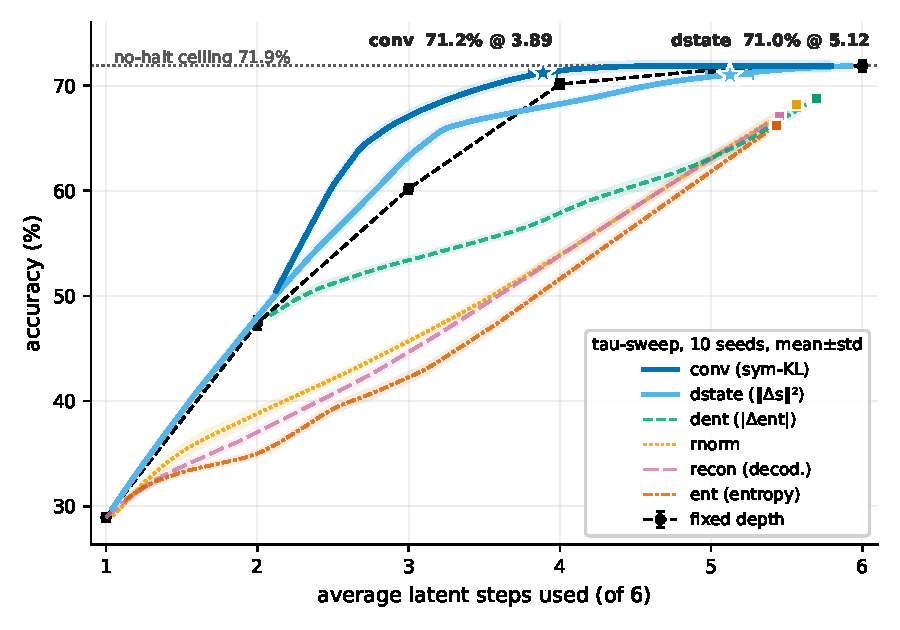
\includegraphics[width=0.78\linewidth]{fig1_bakeoff_band.pdf}
\caption{$\tau$-sweep accuracy-vs-compute curves for all six signals (10-seed
mean$\pm$std bands; no extrapolation beyond each seed's observed range), the
fixed-depth frontier, and each signal's calibrated operating point (star =
convergence winners). Only \sig{conv}/\sig{dstate} reach the no-halt ceiling;
the four magnitude-family signals plateau 3--6pp below it.}
\label{fig:bakeoff}
\end{figure}

Three things stand out. \textbf{(i) A real compute saving.} \sig{conv} reaches
within 1pp of the ceiling at $3.89/6$ steps --- a ${\sim}35\%$ saving --- and
it is \emph{uniform}: per-seed steps lie in $[3.80, 4.07]$ with no bimodality.
\textbf{(ii) The saving carries information.} \sig{conv} beats its within-block
shuffle null by $\mathbf{+7.4}$\textbf{pp} ($71.2$ vs $63.8$), so its halt
decisions depend on the specific example, not a per-position schedule.
\textbf{(iii) Surprise halts prematurely.} The premature-halt fraction per halt
is $0.02$ for \sig{conv} versus $0.50$ for \sig{ent} --- half of every entropy
halt fires on an example that had not yet resolved. \sig{dstate} is the
\emph{safe} convergence signal (premature $0.05$) but more conservative
($5.12$ steps), matching the ceiling with a smaller saving.

\subsection{Why surprise fails: failure decomposition}\label{sec:failure}

The canonical run's own per-example decomposition names the failure. Under each
signal's calibrated $\tau$, \textbf{premature halts} --- halted early and
answered wrong where the full-depth rollout answers right --- hit $5.9\pm0.3\%$
of examples for \sig{ent} and $5.0\pm0.2\%$ for \sig{recon} (decodability),
versus $2.1\pm0.5\%$ for \sig{conv} and $1.9\pm0.5\%$ for \sig{dstate}; per
halt issued, half of entropy's halts are premature ($0.50$ vs \sig{conv}'s
$0.02$; Table~\ref{tab:bakeoff}). And the magnitude signals point the wrong
way: $\mathrm{corr}(\text{answerable}, \text{signal})$ is \emph{negative}
(\sig{ent} $-0.46\pm0.01$, \sig{recon} $-0.18\pm0.02$) --- the signal reads
``confident, stop'' partway through an unresolved multi-hop chain --- while the
convergence signals track answerability weakly \emph{positively} (\sig{conv}
$+0.15\pm0.01$, \sig{dstate} $+0.05\pm0.01$) and simply keep moving until the
computation settles. The retired strong-learner bake-off corroborates
independently (whose \sig{recon} is the \textbf{state-mismatch} form --- a
different scalar, same verdict): 8--9\% early-and-wrong exits for entropy/recon
vs 1--4\% for the convergence family, corr $-0.45$/$-0.25$
(Appendix~\ref{app:weak}). The mechanism is task-dependent --- on multi-hop
MQAR entropy/recon \emph{drift to the budget} past the accuracy peak rather
than halting confident-wrong-early (\S\ref{sec:transfer}) --- but the verdict
is the same: magnitude signals are miscalibrated as halting rules exactly where
the task has depth structure.

\subsection{External transfer: multi-hop associative recall}\label{sec:transfer}

The discrimination reproduces on an external task. On \textbf{multi-hop MQAR}
($H$-hop recall, $H\in1..3$; persist ceiling $41.6\pm0.9\%$), convergence beats
magnitude at \textbf{less than half the compute} ($2.5$ vs $5.4$ steps),
winning on \textbf{all 10 seeds} --- conv$-$entropy $= +2.76\pm0.35$pp,
conv$-$recon $= +2.32\pm0.33$pp (both 10/10); see Table~\ref{tab:mqar}.

\begin{table}[t]
\caption{Multi-hop MQAR transfer (10 seeds; persist ceiling $41.6\pm0.9\%$).}
\label{tab:mqar}
\centering
\small
\begin{tabular}{lll}
\toprule
signal & acc (\%) & avg steps \\
\midrule
\sig{conv}   & $\mathbf{42.3\pm0.9}$ & $2.48\pm0.11$ \\
\sig{dstate} & $42.2\pm0.9$ & $2.72\pm0.20$ \\
\sig{entropy} & $39.5\pm0.8$ & $5.40\pm0.03$ \\
\sig{recon} (state-mism.) & $40.0\pm0.9$ & $5.40\pm0.02$ \\
\bottomrule
\end{tabular}
\end{table}

Halting depth also \textbf{grows with hop count} --- \sig{dstate} mean halt
step $2.75\pm0.12$ ($H{=}1$) $\to$ $3.45\pm0.13$ ($H{=}2$) $\to$ $3.51\pm0.18$
($H{=}3$) --- so the controller spends more steps on harder probes, the
behavior a depth knob should have. The \textbf{single-hop control} is the
informative null: there all four signals are cost-free (\sig{conv} matches the
$68.2\pm0.5\%$ ceiling at $2.53\pm0.30$ steps, ${\sim}58\%$ saved), because
single-hop errors are the ${\sim}30\%$ \emph{unanswerable} probes that are
wrong at any depth --- so early halting is harmless and signal choice does not
matter. Signal choice matters \textbf{exactly when the task has depth
structure}, which is the whole claim.

\subsection{The counterweight}\label{sec:counterweight}

We do not claim the reconstruction family is a bad signal \emph{universally}
--- only for \emph{halting on joint tasks}. On the \textbf{memory-only} rule
task, an independent bake-off (weak learners, stronger nulls) finds that a
reconstruction-family scalar (\textbf{decodability} form) is as good a halting
signal as entropy at matched compute (recon $50.1\pm0.5\%$ @ $2.38$ steps
$\approx$ ent $50.1\pm0.7\%$ @ $2.22$; persist $50.5\pm0.4\%$; steps are
10-seed means). On the \emph{joint} task in the same bake-off, entropy simply
\emph{refuses to halt} ($34.7\%$ @ $9.71$ steps) and only \sig{dstate} yields a
useful operating point ($33.8\%$ @ $6.28$ steps, $-1.3$pp at $63\%$ compute).
Two caveats we keep visible: this recon is the \textbf{decodability} scalar ---
the \emph{same} definition as \S\ref{sec:bakeoff}--\ref{sec:failure}'s
canonical \sig{recon}, and a \emph{different} one from the
\textbf{state-mismatch} recon of \S\ref{sec:failure}'s corroboration and
\S\ref{sec:transfer} (we never treat the two as one signal behaving
inconsistently); and the three bake-off implementations differ in learner and
$\tau$-rule and are reported separately --- \S\ref{sec:bakeoff} is the
canonical comparison (Appendix~\ref{app:weak} for the others). The
counterweight sharpens rather than softens the diagnosis: the write gate's own
signal is fine \emph{for writing}, and even fine for halting when there is no
multi-hop depth to misjudge --- it fails precisely on the joint regime the
unification was supposed to cover.

\section{Discussion}

\paragraph{The diagnosis.} The write gate and the depth knob want
\emph{different observables}. A reconstruction-miss detects ``unknown
content'' --- the right trigger for \emph{writing} to memory. A convergence
observable detects ``computation settled'' --- the right trigger for
\emph{stopping}. These come apart on any task with depth structure, because a
chain can be far from settled while the current readout is confidently (and
wrongly) low-entropy. The one-signal unification is therefore refuted \textbf{in
its literal form}: no single scalar we tested serves both roles, and the two
that halt cost-free (\sig{conv}, \sig{dstate}) have no write role at all.

\paragraph{What we do not claim.} A weaker, interpretive reading --- that
halting and writing are two gradients of one memory loss ($\nabla_s L$ for
depth, $\nabla_W L$ for the write), with $\norm{\Delta s} \approx \eta
\norm{\nabla_s L}$ near a step's fixed point --- is \emph{consistent} with our
data, but we neither test nor claim it: it is near-tautological as stated, and
our experiments neither support nor refute it as a mechanism. Turning it into a
finding requires showing the halt signal \emph{predicts the write magnitude},
which needs interventional, functional-form, cross-regime evidence in a
tractable setting (e.g.\ in-context linear regression) --- future work, and
explicitly out of scope here. We also do not make any write-magnitude claim
from the current probe, which is doubly confounded.

\paragraph{Practical recipe.} If you add halting to a TTT-style memory model:
use a \emph{convergence} observable (readout-KL or latent step norm), calibrate
its threshold on a \emph{held-out} stream by fewest-steps-within-slack, and
validate against a within-block shuffle null. Do \textbf{not} reuse the
write/surprise signal as the halting rule --- it halts confident-and-wrong
exactly on the multi-hop examples where extra depth would have paid off.

\section{Limitations}

\begin{itemize}
  \item \textbf{Mechanism scale.} Models are 0.2--0.9M parameters on synthetic
  tasks; these are mechanism pilots, not LLM-scale evidence.
  \item \textbf{Non-standard MQAR.} Our mini-MQAR uses vocab 64, not the
  standard Zoology config (vocab 8192). A standard-config anchor run is in
  progress. % TODO: replace with mqar8k result when the run completes
  \item \textbf{Compute accounting.} ``Compute'' counts retrieval steps only;
  delta-rule \emph{write} FLOPs are unaffected by halting and not counted.
  \item \textbf{Weak multi-hop learner.} The multi-hop MQAR base learner
  ceilings at $41.6\%$; the \emph{discrimination} is robust across 10 seeds but
  the absolute accuracy is not meaningful.
  \item \textbf{Interpretation, not mechanism.} The ``two gradients of one
  loss'' reading is stated as an untested interpretation (\S5), not a result.
\end{itemize}

\section{Conclusion}

We asked whether one surprise signal can govern both test-time knobs of a
fast-weight memory reasoner, and answered no for the halting half. Across a
canonical 10-seed bake-off on a joint memory+depth task and an external
multi-hop recall transfer, reconstruction-error and entropy thresholds halt
confidently-and-wrong (or refuse to halt), while convergence observables are
the only signals that reach the no-halt ceiling --- the best of them at
${\sim}65\%$ of the compute, uniformly across seeds. Surprise loses,
convergence wins: the write gate and the depth knob want different observables.
We release the bake-off protocol as a reusable recipe for choosing halting
signals in test-time-adaptive models.

\bibliographystyle{plainnat}
\bibliography{references}

\appendix

\section{Signal inventory and the two reconstruction definitions}\label{app:signals}

Different experiments in this project used different scalars for the write gate
and for halting; conflating them is the fastest way to misread the result.
Table~\ref{tab:inventory} is the complete inventory.

\begin{table}[h]
\caption{Which scalar drove what, per experiment. The write gate is
\emph{identical} in every bake-off (the delta-rule reconstruction miss ---
writes were never modified); only the \emph{halting} signal was raced.}
\label{tab:inventory}
\centering
\small
\begin{tabular}{lll}
\toprule
experiment & write gate & halting signal \\
\midrule
depth-only sanity & --- (no memory) & prediction-stability (hindsight convergence) \\
literal-thesis pilot (\sig{ttt}) & recon error (shared) & recon error (shared); task inconclusive \\
memory-only rule task & recon error & readout entropy \\
joint reachability (historical) & recon error & readout entropy \\
retired bake-off (App.~\ref{app:weak}) & recon error (unchanged) & 4 signals; \sig{recon} = \textbf{state-mismatch} \\
weak-learner bake-off (App.~\ref{app:weak}) & recon error (unchanged) & 5 signals; \sig{recon} = \textbf{decodability} \\
\textbf{canonical bake-off (\S\ref{sec:bakeoff})} & recon error (unchanged) & 6 signals; \sig{recon} = \textbf{decodability} \\
MQAR transfer (\S\ref{sec:transfer}) & recon error (unchanged) & 4 signals; \sig{recon} = \textbf{state-mismatch} \\
\bottomrule
\end{tabular}
\end{table}

\paragraph{The two reconstruction definitions.} The \textbf{state-mismatch}
form, $\norm{n(s_{t+1}) - n(r_t)}^2$ (with $n$ a normalization), measures the
disagreement between the updated latent state and the memory read --- the
closest inference-time analogue of the write-side surprise. The
\textbf{vocab-decodability} form, $\min_v \norm{r_t - \mathrm{node}(v)}^2$,
measures how close the read is to \emph{some} vocabulary embedding. The literal
TTT write loss knows the probe's true target and therefore cannot be used as a
halting signal at inference; these two scalars are its self-supervised proxies.
We report them separately everywhere: ``recon halting survives on the
memory-only task but loses on joint tasks'' (\S\ref{sec:counterweight}) is a
statement about the decodability form in both clauses, and the state-mismatch
form independently loses on the joint task (App.~\ref{app:weak}) and on
multi-hop MQAR (\S\ref{sec:transfer}) --- the verdict is the same for both, but
they are never pooled as one signal.

\section{The two non-canonical bake-offs}\label{app:weak}

Two independent bake-off implementations preceded the canonical run of
\S\ref{sec:bakeoff}. They differ from it (and from each other) in base learner,
$\tau$-selection objective, and \sig{recon} definition, so we report them
separately and never merge their tables; they matter because they
\emph{independently converge} on the same verdict.

\paragraph{B.1 Retired strong-learner bake-off (state-mismatch recon,
argmax-$\tau$).} Same task and learner class as \S\ref{sec:bakeoff} (persist
ceiling $72.0\pm0.6\%$, $T{=}6$), but $\tau$ chosen by \emph{argmax calibration
accuracy} and \sig{recon} in the \textbf{state-mismatch} form
(Table~\ref{tab:retired}). The convergence family preserves accuracy
($-0.0$pp); entropy/recon lose $5.6$pp by exiting early-and-wrong on 8--9\% of
examples, with \emph{negative} corr(answerable, signal). The $\dagger$ step
counts are $\tau$-rule artifacts dissolved in Appendix~\ref{app:tau}.

\begin{table}[h]
\caption{Retired bake-off (10 seeds, held-out argmax-accuracy $\tau$,
\sig{recon} = state-mismatch). Persist ceiling $72.0\pm0.6\%$.}
\label{tab:retired}
\centering
\small
\begin{tabular}{lllll}
\toprule
signal & acc (\%) & avg steps & early-wrong & corr(ans, sig$_0$) \\
\midrule
\sig{dstate} & $\mathbf{72.0\pm0.6}$ & $5.93\pm0.06\,\dagger$ & $\mathbf{1.1\%}$ & $+0.05$ \\
\sig{conv}   & $71.9\pm0.6$ & $5.00\pm0.58\,\dagger$ & $3.6\%$ & $+0.14$ \\
\sig{entropy} & $66.4\pm0.9$ & $5.44\pm0.04$ & $8.5\%$ & $-0.45$ \\
\sig{recon} (state-mism.) & $66.3\pm0.7$ & $5.39\pm0.03$ & $8.8\%$ & $-0.25$ \\
\bottomrule
\end{tabular}
\end{table}

\paragraph{B.2 Weak-learner bake-off with stronger nulls (decodability recon,
slack-$\tau$).} An independent implementation on the \emph{original} (no
curriculum fix) tasks, with the within-block shuffle null and slack-based
held-out $\tau$ that the canonical run later adopted (Table~\ref{tab:weak}).
It adds the two facts the strong-learner runs cannot: (i) on the
\textbf{memory-only} rule task a reconstruction-family scalar (decodability) is
as good a halting signal as entropy --- the failure is specific to \emph{joint}
tasks; (ii) on weak-learner joint reachability ($T{=}10$), entropy does not
\emph{hurt} --- it simply refuses to halt --- and only \sig{dstate} offers a
useful operating point. (This implementation also raced \sig{rnorm} and
\sig{dent}; both behave like the magnitude family and are omitted here for
space.)

\begin{table}[h]
\caption{Weak-learner bake-off (10 seeds, slack-based held-out $\tau$,
\sig{recon} = decodability).}
\label{tab:weak}
\centering
\small
\begin{tabular}{llllp{4.2cm}}
\toprule
task (persist) & signal & acc (\%) & steps & verdict \\
\midrule
rule ($50.5\pm0.4\%$) & \sig{ent} & $50.1\pm0.7$ & $2.22$ & works \\
rule & \sig{recon} (decod.) & $50.1\pm0.5$ & $2.38$ & $\approx$ \sig{ent}: recon-halting survives on the memory-only task \\
rule & \sig{dstate} & $50.3\pm0.6$ & $\mathbf{1.90}$ & best \\
\midrule
reachp ($35.1\pm0.7\%$) & \sig{ent} & $34.7\pm0.6$ & $9.71$ & refuses to halt (safe but useless) \\
reachp & \sig{recon} (decod.) & $31.7\pm0.6$ & $8.39$ & $-3.4$pp, $\tau$ fallback \\
reachp & \sig{dstate} & $33.8\pm0.6$ & $\mathbf{6.28}$ & only useful operating point ($-1.3$pp at $63\%$ compute) \\
\bottomrule
\end{tabular}
\end{table}

\section{$\tau$-rule ablation: argmax-accuracy vs fewest-steps-within-slack}\label{app:tau}

The retired bake-off (App.~\ref{app:weak}, B.1) and the canonical run
(\S\ref{sec:bakeoff}) share the task family, learner class
(curriculum{+}aux, $d{=}256$), budget ($T{=}6$), and the \sig{conv}/\sig{dstate}
signals; the consequential difference for those two signals is the
\textbf{$\tau$-selection objective} on the held-out calibration stream. That
swap alone changes the apparent character of the result
(Table~\ref{tab:taurule}):

\begin{table}[h]
\caption{The same two convergence signals under the two $\tau$ rules
(10 seeds each; independent eval draws).}
\label{tab:taurule}
\centering
\small
\begin{tabular}{lll}
\toprule
 & argmax calibration accuracy (B.1) & fewest steps within 1pp slack (\S\ref{sec:bakeoff}) \\
\midrule
\sig{conv} steps & $5.00\pm0.58$ --- \textbf{bimodal}: 7 seeds at & $3.89\pm0.09$ --- \textbf{uniform}, \\
 & $4.35$--$4.77$, 3 seeds at $5.85$--$5.91$ & per-seed range $[3.80, 4.07]$ \\
\sig{dstate} steps & $5.93\pm0.06$ --- pinned at the budget & $5.12\pm0.15$ --- actually halts \\
 & (``declines to halt'') & \\
\bottomrule
\end{tabular}
\end{table}

The diagnosis is simple: for an accuracy-preserving signal the calibration
accuracy-vs-$\tau$ curve is \emph{flat on top} --- many thresholds tie within
noise --- so argmax picks an arbitrary point on the plateau, and the resulting
operating point lands anywhere between ``halts early'' and ``never halts.''
Fewest-steps-within-slack breaks the tie in the direction the halting question
actually asks (least compute at preserved accuracy) and pins the operating
point, dissolving both the \sig{conv} bimodality and the \sig{dstate}
conservatism. Under the argmax rule we would have (and initially did) read
these artifacts as properties of the signals.

The practical lesson for anyone running a halting bake-off: the
$\tau$-selection objective is \emph{part of the protocol}, not an
implementation detail --- report it, and prefer a compute-aware rule when the
claim is about compute.

\end{document}
